\chapter{Application}
\label{chap:anwendung}

This chapter will explain how to use the application which was developed in the context of this thesis. It has the working title \textit{Doingnotes}. Installation and operation of all functionality are documented within.

\section{Installation}
\label{sec:installation}

The next two sections will describe the installation of CouchDB and the deployment of the application.

\subsection{CouchDB}

First, CouchDB has to be installed on all computers that will use Doingnotes. CouchDB is extensively discussed in section \ref{sec:technisch-couchdb}. Since earlier versions do not support continuous replication which is necessary for Doingnotes, CouchDB is needed in version 0.11.0 or higher.

CouchDB will run on most popular desktop operating systems and some established mobile platforms. Currently, the latter include Google Android (\cite{couchmobile:android}) and Nokia MeeGo (formerly Maemo) (\cite{couchmobile:nokia1}), \cite{couchmobile:nokia2}). Recently, Palm announced that the next version of its mobile Operating System WebOS would also come with a CouchDB installation (\cite{couchmobile:webos}).

For some desktop operating systems, pre-compiled CouchDB binaries exist. All dependencies are contained within. If CouchDB is installed from the source code, these dependencies have to be resolved manually. Amongst other things, CouchDB requires Erlang \cite{erlang:homepage}, OpenSSL \cite{openssl} and Spidermonkey \cite{spidermonkey} to be installed. More details can be found in section \ref{subsec:einsatz}.

The quickest way to get CouchDB up and running on Mac OS X is by downloading \textit{CouchDBX}: \enquote{The one-click CouchDB package for the Mac} \cite{couch:couchdbx}. A binary installer is also available for Windows systems \cite{couch:windows}. Some Linux distributions have already included CouchDB in their software repositories; e.g. in newer Ubuntu versions, CouchDB can be installed using the packaging tool \textit{apt}.

Doingnotes will work fine using the current versions of the three aforementioned binaries, and they are by all means recommended for end users. Developers, however, may want to install CouchDB directly from the source code. In doing so, they may retrieve the latest version from the Subversion \cite{couch:svn} or Git \cite{couch:github} repositories. More detailed instructions on how to install CouchDB on different operating systems and distributions can be found in the CouchDB Wiki \cite{couch:installation}. How CouchDB is started depends on the operating system. Again, more details can be found in the Wiki.

\subsection{Deployment}
\label{subsec:deployment}

The next step involves installing CouchApp \cite{couch:couchapp}. CouchApp was introduced in section \ref{subsec:couchapp}. CouchApp allows the application to be easily deployed into the CouchDB instance. CouchApp assumes that a recent version of Python is installed \cite{python:homepage}: it requires Python's {\fontfamily{pcr}\selectfont easy\_install} module \cite{python:easy} in order to download and install CouchApp, also a Python package.

It is necessary to alter {\fontfamily{pcr}\selectfont .couchapprc} in the project directory to deploy the design documents (i.e. the code) into the CouchDB instance; the entry {\fontfamily{pcr}\selectfont default} must point to the running CouchDB instance (see listing \ref{code:couchapprc}). Afterwards, {\fontfamily{pcr}\selectfont couchapp push} has to be called from here in order to deploy the application into the database and make it executable.

The application can be accessed using a browser that meets the discussed in section \ref{subsec:nochanges}. Firefox \cite{firefox} 3.5 or higher is recommended.


\section{Operation}
\label{sec:bedienung}

\subsection{Basic functionality}

The application allows lines to be sorted and saved inside the outline. The page {\url{http://localhost:5984/doingnotes/\_design/doingnotes/index.html}} is the main page. As all other pages, it contains a navigation bar and a content area. The main page can be reached from anywhere in the application by clicking on the \enquote{Outlines} link. The content area lists existing outlines (see fig. \ref{fig:outline-list}). Next to the title of every outline is the time and date of creation. If there are no outlines available, the overview displays the text \enquote{You have no outlines yet}. On the right-hand side, there are some hints on how to create an outline.

\medskip
\begin{figure}[ht] 
  \begin{center}
    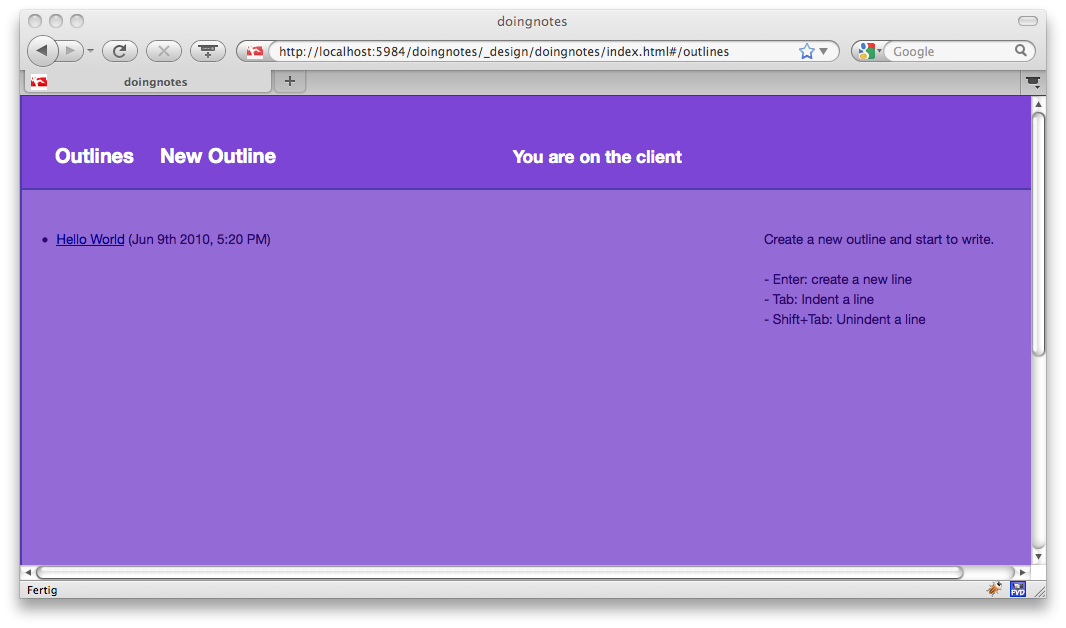
\includegraphics[width=\textwidth]{grafik/screenshot-outline-list} 
  \end{center}
  \caption{Screenshot: list of outlines}
  \label{fig:outline-list} 
\end{figure}

In order to create a new outline, the user has to click \enquote{New Outline}. Titles must be at least three characters long and may only contain alphanumeric characters, blanks and hyphens. The title does not have to be unique as outlines are referenced by their ID. Erroneous input as well as clues about conflicts and replication status are displayed near the application's upper border and fade out after a few seconds. The signal colours of the notification indicate errors (red) or notices (green).

\medskip
\begin{figure}[ht] 
  \begin{center}
    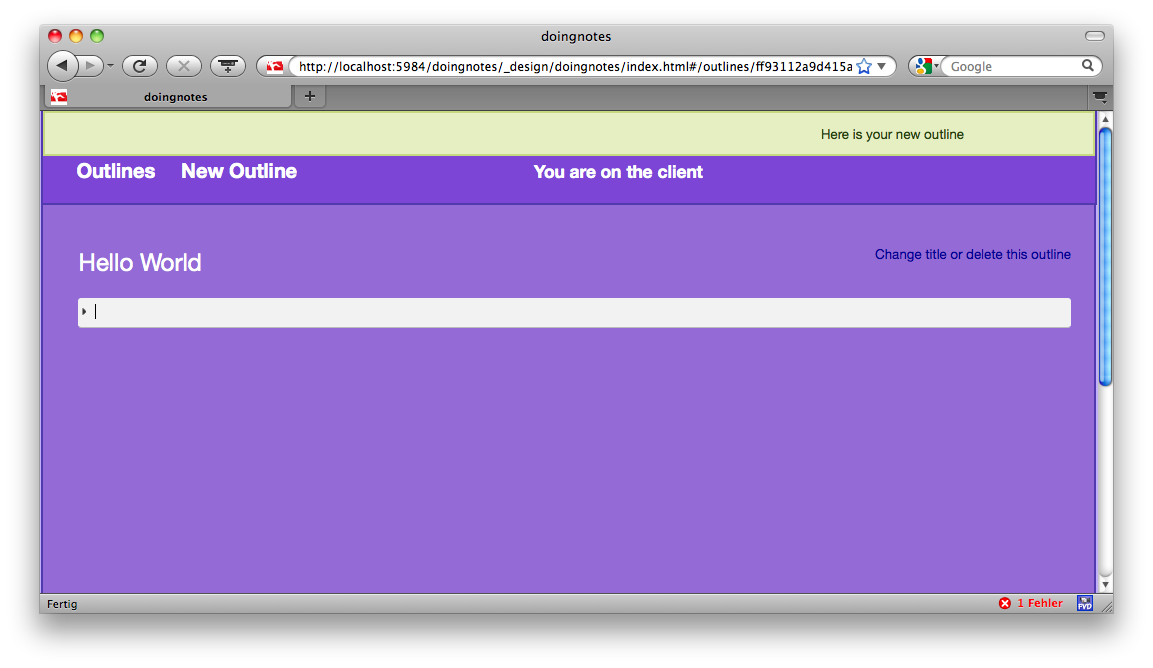
\includegraphics[width=\textwidth]{grafik/screenshot-new-outline} 
  \end{center}
  \caption{Screenshot: newly created outline}
  \label{fig:new-outline} 
\end{figure}

When an outline has been created (see fig. \ref{fig:new-outline} it is immediately opened. Text can be entered into the first line. If the text's length exceeds that of the line, the line will automatically grow along. If \textbf{Enter} is hit, a new line will be created. An animated throbber in the right-upper corner indicates that the line is still being created.

Navigating between the lines can be done using the \textbf{arrow keys}. The \textbf{Tab} key indents a line, creating hierarchy between the entries. A line can be indented as long as there is a line with the next higher indentation level directly above it. \textbf{Shift + Tab} outdents a line. This keystroke will not work for lines on the first level. When manually resolving conflicts (see section \ref{subsec:conflres-anwendung}), the \textbf{Tab} or \textbf{Shift + Tab} keys allow jumping back and forth between conflict fields.

\enquote{Change title or delete this outline} points to the edit outline page (see fig. \ref{fig:edit-outline}). Here, the outline's title may be changed. Clicking the \enquote{Delete this outline} button will promptly delete the outline.

\medskip
\begin{figure}[ht] 
  \begin{center}
    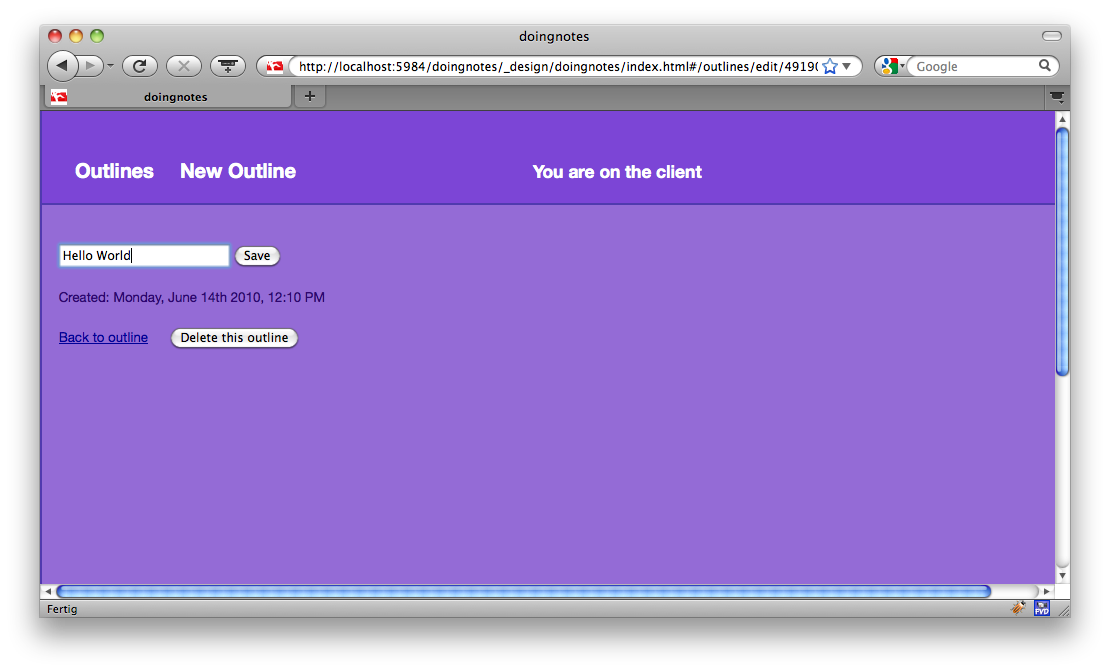
\includegraphics[width=\textwidth]{grafik/screenshot-edit-outline} 
  \end{center}
  \caption{Screenshot: editing the outline title}
  \label{fig:edit-outline} 
\end{figure}

Now that the user has familiarised herself with the application as a single-user system, the following sections will introduce the application's multi-user features.

\subsection{Replication}

In order to use replication and conflict resolution, Doingnotes must run in more than one CouchDB instance; i.e. Doingnotes has to be deployed onto a server to be able to use all its features. The CouchDB instance on the server will hereinafter be called the \enquote{server}; the instance on the user's computer is the \enquote{client}.

Server and client can also run on the same computer. In order to test replication, the same outline has to be opened in more than one browser window. In doing so, one can monitor how updates are automatically replicated to the server (or to other clients) and how the conflict resolution mechanism kicks in. Whether the server is on the same computer or not, its URL has to be correctly entered into the configuration file {\url{/_attachments/app/config/config.js}}.

For operation on a single computer, two CouchDB instances have to be installed, as described in section \ref{subsec:lounge-install} (see also \cite{lounge:twoinstances}). In this set-up, the server URL in {\url{/\_attachments/app/config/config.js}} must point to {\url{http://localhost:5984}}.

The CouchDB instances on ports 5984 and 5985 (client and server) are opened in two browser windows. For extra clarity, the navigation bar indicates which browser window the user is currently working in: it will either read \enquote{You are on the client} or \enquote{You are on the server}. The same outline is now opened in each of the two windows. If something is changed in the server window, the user in the client window is notified of this: \enquote{Replication has brought updates.} (see fig. \ref{fig:outline-note}). Clicking \enquote{View them.} reloads the page, displaying the update (see fig. \ref{fig:outline-updated}).


\medskip
\begin{figure}[ht]
  \begin{center}
  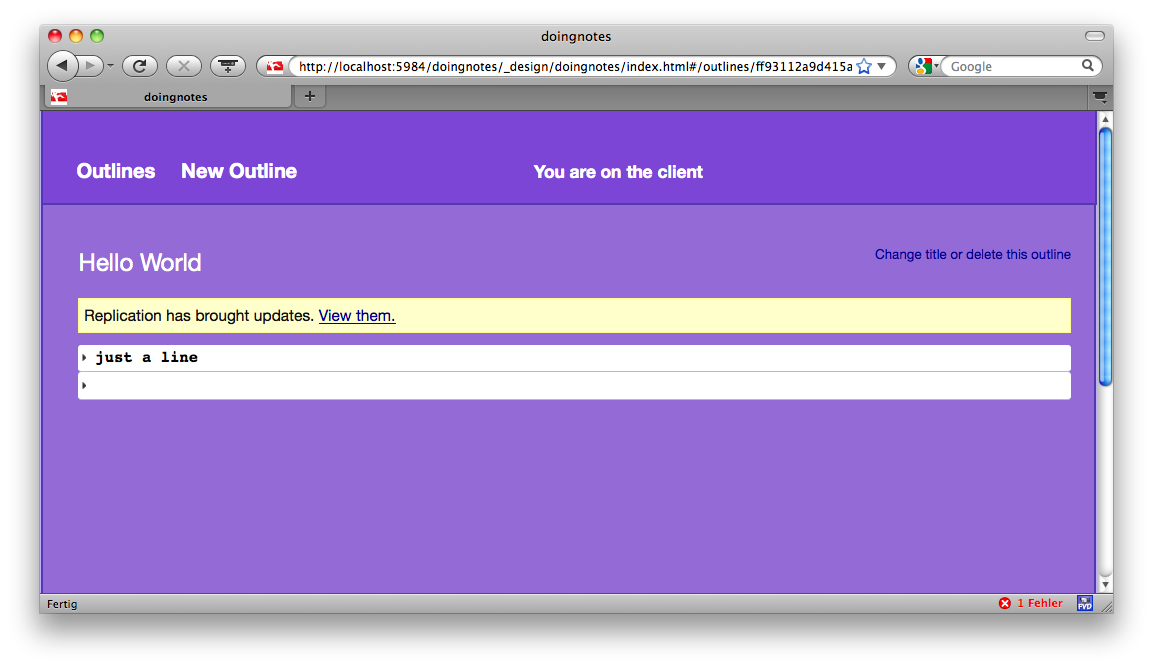
\includegraphics[width=\textwidth]{grafik/screenshot-outline-replication-note}
  \end{center}
  \caption{Screenshot: an outline with notification of replication}
  \label{fig:outline-note}
\end{figure}


\medskip
\begin{figure}[ht]
  \begin{center}
  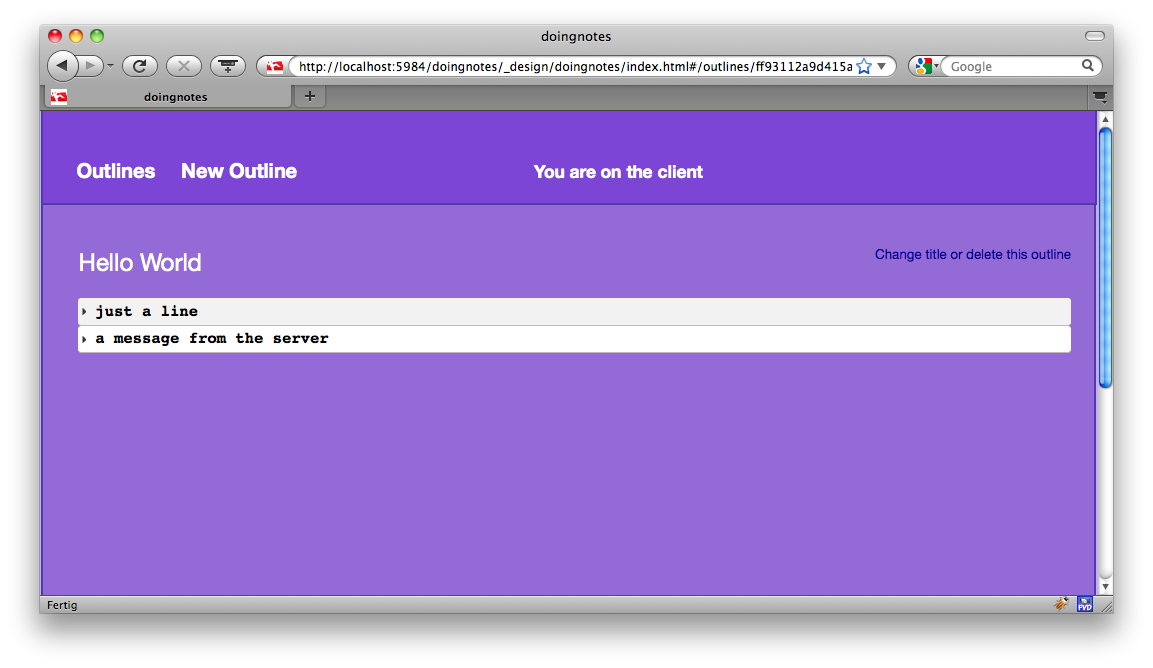
\includegraphics[width=\textwidth]{grafik/screenshot-updated-outline}
  \end{center}
  \caption{Screenshot: the outline after updating}
  \label{fig:outline-updated}
\end{figure}

If the connection drops or if the user intentionally disconnects in the meantime, the replication can be restarted by simply reloading the page.


\afterpage{\clearpage}

\subsection{Conflict handling}
\label{subsec:conflres-anwendung}

If replication caused no conflicts, its results are simply shown. There are two types of conflicts the application was programmed to deal with: \textit{append conflicts} and \textit{write conflicts} (cf. sections \ref{subsec:appendkonfl-arch} and \ref{subsec:writekonfl-arch}). An append conflict occurs when more than one user simultaneously add a new line in the same spot. A write conflict occurs if the contents of a line are modified by two or more users simultaneously.

\subsubsection{Creating conflicts for testing purposes}

A write conflict can be provoked by following these steps one after another (client and server may be swapped around):

\begin{itemize}
\item stop the CouchDB server instance
\item enter text in the client window
\item stop the client instance
\item start the server instance
\item enter text in the server window
\item start the client instance
\end{itemize}

To ensure that conflicts occur, the instances have to be shut down or started completely before proceeding to the next step. Only this will interrupt the automatic replication long enough for a conflict to occur.

In order to provoke an append conflict, a new line has to be added after the same line in both windows, instead of entering text. The system can also deal with both conflict types occurring in the same line.


\subsubsection{Handling}


\minisec{Append conflicts}

If an update to the server causes an append conflict, it is automatically resolved by the server. A notification \enquote{Replication has automatically solved updates} is shown and in addition, the affected lines are highlighted in green (see fig. \ref{fig:appendconflict}).


\medskip
\begin{figure}[ht] 
  \begin{center}
  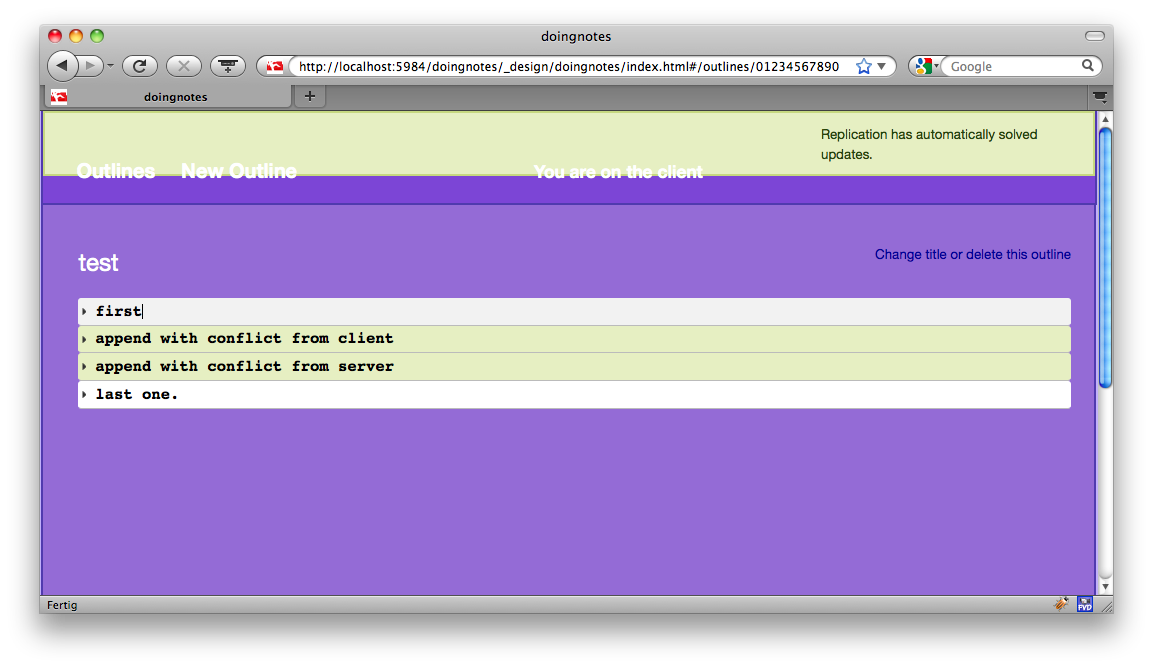
\includegraphics[width=\textwidth]{grafik/screenshot-append-conflict} 
  \end{center}
  \caption{Screenshot: automatically resolved append conflict}
  \label{fig:appendconflict}
\end{figure}


The conflict is resolved by putting the line that was added first before the one that was added last. However, the order is not reliable since the clocks on two systems are not necessarily synchronised. If conflict resolution happens simultaneously on two computers (clients), each computer sorts the lines in the same way, preventing new conflicts from being produced by the conflict resolution process. More details about this process can be found in section \ref{subsec:appendconflict-implementierung}.

\minisec{Write conflicts}

If an update causes a write conflict to occur, the user has to decide which version shall remain in the system and which one should be rejected. The user may also manually merge the versions. A notification \enquote{Replication has caused one or more conflicts.} is displayed. Additionally, the affected lines are coloured red (see fig. \ref{fig:writeconflict}).

\medskip
\begin{figure}[ht] 
  \begin{center}
  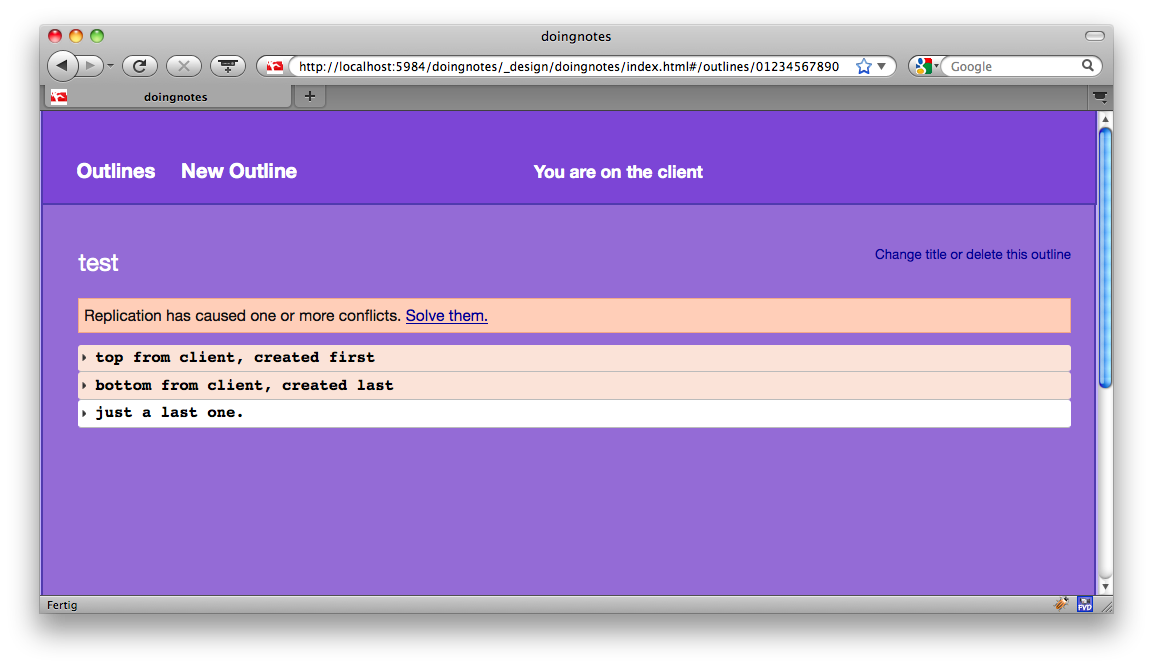
\includegraphics[width=\textwidth]{grafik/screenshot-write-conflict} 
  \end{center}
  \caption{Screenshot: unresolved write conflict notification}
  \label{fig:writeconflict} 
\end{figure}

The write conflict must be resolved manually. The user is therefore presented with a mask which displays both versions for every conflicting line (see fig. \ref{fig:writeconflict-solving}). She may now decide which one to keep and even freely edit the line before saving. Distinct captions on the save buttons (\enquote{Keep overwritten version} and \enquote{Keep winning version}) indicate which version was elected winner by CouchDB's internal conflict resolution mechanism. More details can be found in section \ref{subsec:writeconflict-implementierung}.

\medskip
\begin{figure}[ht] 
  \begin{center}
  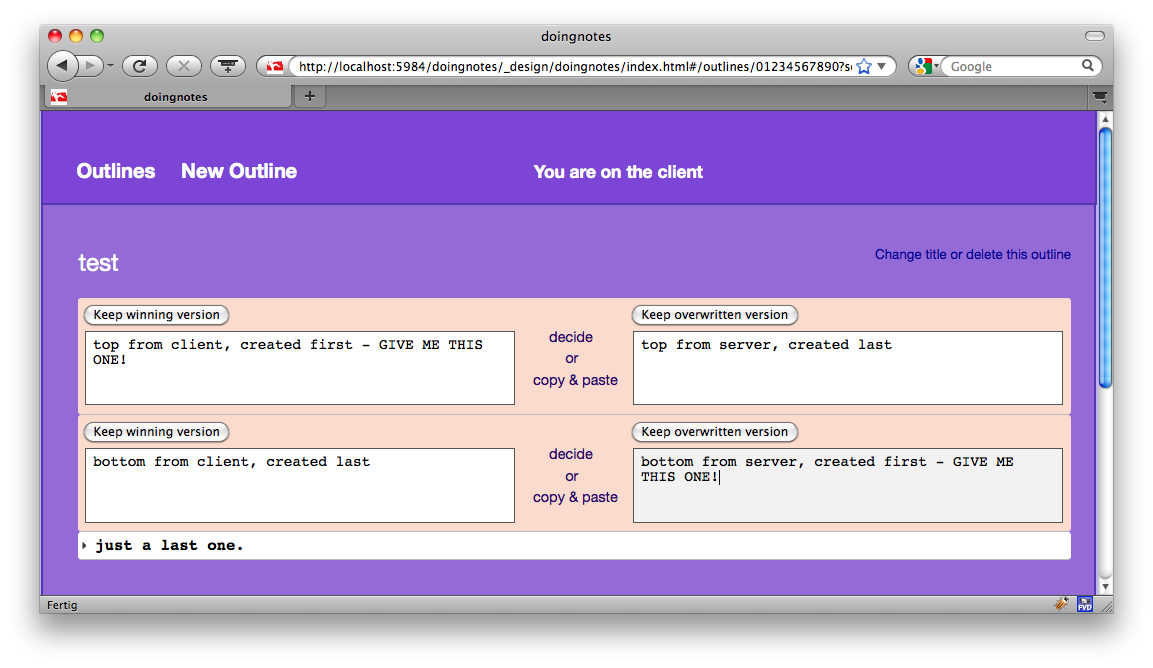
\includegraphics[width=\textwidth]{grafik/screenshot-write-conflict-solving} 
  \end{center}
  \caption{Screenshot: manual write conflict resolution}
  \label{fig:writeconflict-solving}
\end{figure}


The conflicts are thus resolved line by line. After saving a version of a line it is conflict-free. The conflict resolution mask is hidden for every line and the winning line is shown instead. If all conflicts have been resolved the user is notified about this, as shown in figure \ref{sec:piffpaff}.

\medskip
\begin{figure}[ht] 
  \begin{center}
  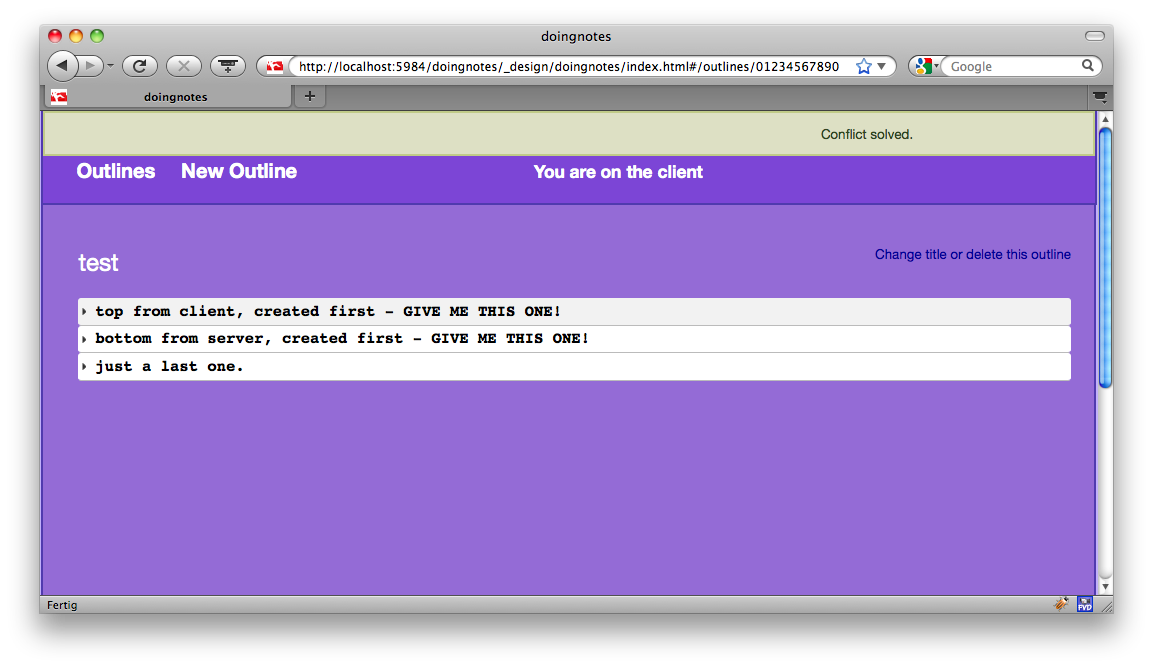
\includegraphics[width=\textwidth]{grafik/screenshot-write-conflict-solved} 
  \end{center}
  \caption{Screenshot: write conflict resolved}
  \label{sec:piffpaff} 
\end{figure}

\afterpage{\clearpage}

\subsection{Assistance in provoking conflicts}
\label{subsec:hilfestellung}

Some macros were created to make generating conflicts easier. These put the database in a well defined state. It is not possible to manually provoke conflicts in CouchDB. Therefore, the macros simply automate the steps described in the previous section. The macros have been implemented as \textit{Rake tasks}. Rake is a build tool written in Ruby. It is similar to the make program: commandos are executed under certain conditions and in a certain order \cite{rake:website}. Users can create their own command batches in Ruby syntax, the so-called Rake tasks.

Prior to using Rake, Ruby \cite{ruby:homepage} must be installed. The Rakefile must be modified to contain the correct URLs and ports of the CouchDB instances. Client and Server are pre-set to run on localhost on ports 5984 and 5985.

The {\fontfamily{pcr}\selectfont Rakefile} file in the project's root directory contains the following Rake tasks:

\begin{description}
  \item[couch:recreate\_host] \textit{Resets} (Deletes and recreates) the database; The application is deployed into the CouchDB client instance
  \item[couch:recreate\_server] Resets the database; the application is deployed into the CouchDB server instance
  \item[couch:wait] Waits two seconds before proceeding to the next step
  \item[couch:start\_host] Starts the CouchDB client instance
  \item[couch:start\_server] Starts the CouchDB server instance
  \item[couch:stop\_host] Stops the client instance
  \item[couch:stop\_server] Stops the server instance
  \item[couch:writeconflict] Resets the database; generates an outline with a write conflict
  \item[couch:twowriteconflicts] Resets the database; generates an outline with two write-conflicts
  \item[couch:appendconflict] Resets the database; generates an outline with an append conflict
  \item[couch:appendandwriteconflict] Resets the database; generates an outline with an append and a write conflict
\end{description}

For the tasks referring to client or server, there are also steps that execute the tasks on both instances simultaneously.